\section{有效电阻与生成树}
\label{sec:graph-sparsification-resistance-trees}

如果只能保留少量边而仍要保持连通，一棵生成树是边数最少的选择。桥一旦丢掉，两侧就断开了——每棵生成树都必须包含桥。团内的边有许多替代路径，选树时可以在它们之间换用。一条边越频繁地出现在随机生成树中，它对保持连通就越重要，抽边时应当给它更大的机会。

这种"出现在生成树中的概率"可以用第~\ref{sec:graph-effective-resistance}节的有效电阻来计算。下面先定义加权生成树的概率，再从改变一条边的电导入手，把这个概率与电导乘电阻联系起来。

\subsection{边的生成树比例}
\label{sec:graph-tree-edge-probability}

设$\mathcal G$连通。对于一棵生成树$T$，把树上各边的电导相乘，得到树权$w(T)$。所有生成树的权求和记为$Z$。在有限的生成树集合上，按权成比例的概率抽一棵树，即
\begin{equation}
w(T)=\prod_{e\in T}c_e,
\qquad
Z=\sum_T w(T),
\qquad
\mathbb P(T)=\frac{w(T)}{Z}.
\label{eq:graph-weighted-tree-distribution}
\end{equation}
当所有电导相等时，每棵生成树的权相同，这就退化为等概率抽取。

一条边$e$出现在随机生成树中的概率，是所有含$e$的树各自概率之和。下面证明这个概率恰好等于$c_eR_e$。

\begin{theorem}[生成树的边包含概率]
\label{thm:graph-tree-edge-probability}
对具有正边权的连通图，按式~\eqref{eq:graph-weighted-tree-distribution}抽取生成树。每条边$e$的包含概率为
\begin{equation}
\mathbb P(e\in T)=c_eR_e.
\label{eq:graph-tree-edge-probability}
\end{equation}
\end{theorem}

证明的思路是：把一条边的电导稍微增大，看树权总和怎样变化。直接累加会数到所有含该边的树，用矩阵树定理则会引出约化拉普拉斯的逆。两种方法算的是同一个增量，比较一次项系数就得到结论。

\begin{proof}
把边$e$的电导从$c_e$改成$c_e+t$，其中$t$足够小以保持正权。改变后的树权总和记为$Z(t)$。

一棵包含$e$的生成树，原先的权中有一个因子$c_e$。其余因子的乘积是$w(T)/c_e$，不含$e$的因子不受$t$影响。把$c_e$增加$t$后，这棵树的权变成$(c_e+t)\cdot w(T)/c_e=w(T)+tw(T)/c_e$，增量为$tw(T)/c_e$。

一棵不含$e$的生成树没有这个因子，权保持原值。把所有受影响的树的增量加起来，得到
\[
Z(t)=Z(0)+\frac{t}{c_e}\sum_{T\ni e}w(T).
\]
这是从直接累加树权得到的结果。

接下来用矩阵树定理算同一个$Z(t)$。选一个顶点接地，把拉普拉斯矩阵删去对应行和列，记所得约化矩阵为$\widetilde{\bm L}$。同时把边$e$对应的关联列$\bm b_e$删去该坐标，得到$\tilde{\bm b}_e$。

原拉普拉斯矩阵是各边外积项的和。增大$c_e$时，只有边$e$的外积项增加$t$倍。删去接地行列后，增量为$t\tilde{\bm b}_e\tilde{\bm b}_e^\top$。因此第~\ref{chap:graph-laplacian-matrix}章的矩阵树定理给出
\[
Z(t)=\det(\widetilde{\bm L}+t\tilde{\bm b}_e\tilde{\bm b}_e^\top).
\]

原图连通时$\widetilde{\bm L}$正定，可以在左右两侧各提出$\widetilde{\bm L}^{1/2}$：
\[
\widetilde{\bm L}+t\tilde{\bm b}_e\tilde{\bm b}_e^\top
=\widetilde{\bm L}^{1/2}
  (\bm I+t\bm v\bm v^\top)\widetilde{\bm L}^{1/2},
\]
其中$\bm v=\widetilde{\bm L}^{-1/2}\tilde{\bm b}_e$。取行列式后，外面的两个$\widetilde{\bm L}^{1/2}$贡献$\det\widetilde{\bm L}=Z(0)$，只剩下中间部分的行列式。

矩阵$\bm v\bm v^\top$是秩一的：它把与$\bm v$正交的方向原封不动保留，把$\bm v$方向的长度乘以$\lVert\bm v\rVert_2^2$。因此$\bm I+t\bm v\bm v^\top$在$\bm v^\perp$上的特征值都是一，在$\bm v$方向上的特征值是$1+t\lVert\bm v\rVert_2^2$。将所有特征值相乘，
\[
Z(t)=Z(0)\bigl(1+t\,\tilde{\bm b}_e^\top\widetilde{\bm L}^{-1}\tilde{\bm b}_e\bigr).
\]

这里乘在$t$前面的二次型有清楚的物理含义。设边$e$从$u$记向$v$。在$u$注入单位电流、在$v$取出单位电流时，全图的右端是$\bm b_e=\bm e_u-\bm e_v$。接地后解$\widetilde{\bm L}\tilde{\bm x}=\tilde{\bm b}_e$，得到保留顶点的电势$\tilde{\bm x}=\widetilde{\bm L}^{-1}\tilde{\bm b}_e$。再用$\tilde{\bm b}_e^\top$乘这个解，取出的是$u$点电势减去$v$点电势（接地点的电势按零计）。对单位电流，这个电势差恰好就是有效电阻$R_e$。

两种计算对每个足够小的$t$都给出相同的$Z(t)$。比较一次项系数，得到
\[
\frac{1}{c_e}\sum_{T\ni e}w(T)=Z(0)\,R_e.
\]
两边乘以$c_e$并除以$Z(0)$，左端变成所有含$e$的树的总概率：$\mathbb P(e\in T)=c_eR_e$。
\end{proof}

\begin{example}[四点五边图的全部生成树]
\label{ex:graph-sparsification-trees}
取四点环加对角线$13$的单位权图。从环上删去任一条边就得到一条路径，共有四种删法。加上对角边后，顶点$2$从边$12,23$中选一条接入，顶点$4$从边$34,41$中选一条接入，还能再产生四棵树。图~\ref{fig:sparsification-spanning-trees}把不含和含对角边的两组树分开画出。
\end{example}

\begin{BookInlineFigure}
  \centering
  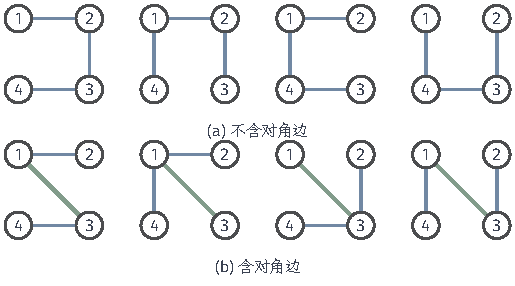
\includegraphics{figures/03-graphs/05-matrices-and-spectra/tikz/sparsification-spanning-trees/figure.pdf}
  \caption{四点五边图的八棵生成树。上排由四环各删去一条边得到，下排固定边$13$后分别把顶点$2$和$4$接到$13$的一个端点。}
  \label{fig:sparsification-spanning-trees}
\end{BookInlineFigure}

八棵树的权都是一。以边$12$为例：不含对角边的四棵树中，有三棵包含$12$（只有删去$12$的那棵不含）。含对角边的四棵树中，有两棵让顶点$2$通过$12$接入。因此$12$在八棵树中出现五次，概率为$5/8$。其余环边同理。对角边$13$出现在第二组全部四棵树中，概率为$1/2$。

电导都是一，所以包含概率$c_eR_e$就等于有效电阻$R_e$。也可以直接用并联公式核对对角边$13$：两端之间有一条电阻为一的直达支路，还有两条各走两条边、电阻为二的绕行支路。三条支路并联后的总电导为$1+1/2+1/2=2$，有效电阻为$1/2$。

\paragraph{桥与对称边}

两个极端的例子可以帮助建立直觉。桥是两侧之间唯一的边，因此每棵生成树都包含它，$c_eR_e=1$。在另一个极端，单位权完全图$K_n$的所有边完全对称，而每棵生成树只用$n-1$条边。把总共$n-1$次出现均分给$\binom n2$条边，每条的包含概率为$2/n$。这两个例子说明，同样的电导可以对应很不同的包含概率，差别来自边在整张图连通结构中的位置。

\subsection{Foster定理}
\label{sec:graph-foster-theorem}

每条边的$c_eR_e$给出一个零到一之间的数。要把这些数变成抽样概率，还需要知道它们的总和是多少。

\begin{theorem}[Foster定理]
\label{thm:graph-foster-theorem}
对$n$个顶点的连通正权图，
\begin{equation}
\sum_{e\in E}c_eR_e=n-1.
\label{eq:graph-foster-sum}
\end{equation}
\end{theorem}

\begin{proof}
对每条边$e$定义随机变量$I_e(T)$：若树$T$含$e$则取一，否则取零。把所有边的$I_e(T)$加起来，就是这棵树$T$的边数。不管抽到哪棵生成树，它都恰好有$n-1$条边，因此
\[
\sum_{e\in E} I_e(T)=n-1.
\]
对等式两边取期望。右边仍是常数$n-1$。左边每个零一变量的期望等于它取一的概率，也就是边$e$出现在随机树中的概率。由式~\eqref{eq:graph-tree-edge-probability}代入，
\[
\sum_{e\in E}\mathbb P(e\in T)
=\sum_{e\in E}c_eR_e=n-1.
\]
这里把各边概率相加是为了算一棵树的平均边数，同一棵树可以同时包含很多条边。
\end{proof}

式~\eqref{eq:graph-foster-sum}称为\term{Foster定理}（Foster's theorem）。在四点五边例中，四条环边各有$c_eR_e=5/8$，对角边为$1/2$，总和$4\times(5/8)+1/2=3=n-1$。

同一个总和也可以用迹来验证。利用$R_e=\bm b_e^\top\bm L_G^\dagger\bm b_e$和$\bm L_G=\sum_e c_e\bm b_e\bm b_e^\top$，交换求和与迹的次序，
\[
\sum_{e\in E}c_eR_e
=\operatorname{tr}\Bigl(\bm L_G^\dagger
   \sum_{e\in E}c_e\bm b_e\bm b_e^\top\Bigr)
=\operatorname{tr}(\bm L_G^\dagger\bm L_G).
\]
乘积$\bm L_G^\dagger\bm L_G$是到$\bm 1^\perp$上的正交投影——它在这个$n-1$维子空间上恒等，在常向量方向上为零。投影的迹等于投影空间的维数$n-1$。

若图有$k$个连通分量，可在每个正权分量中分别计算。所有分量的生成树合起来构成生成森林，总边数为$n-k$。每条正权边的电阻仍然在它所在的分量内定义，孤点不贡献任何边。
